\subsection*{Определение гильтертового пространства.}

\noindent \textasteriskcentered~Полное, бесконечномерное, унитарное пространство назывется \textit{пространством Гильберта} или \textit{гильбертовым пространством}.

\smallskip
\noindent \textasteriskcentered~$H$ - гильбертовое пространство, пространство в котором определено скалярное произведение $(x, y)$, которое позволяет говорить об 
ортогональности точек, 
понятие нормы $\norm{x} = \sqrt{(x, x)}$ и пространство является полным или Банаховым ($x_n - x_m \to 0 \Rightarrow \exists \lim x_n$).

\bigskip
\noindent \textasteriskcentered~Пусть $H_1$ - подпростраство в $H$. Пусть $A \subset H$, тогда $A^{\bot} = \{ x \in H : x \bot a, \forall a \in A\}$.
Получившееся множество, проходящее через нуль, называется \textit{ортогональным дополнением} для множества $A$. $A$ - может быть любым, однако $A^\bot$ всегда подпространство $H$.

\begin{tikzpicture}[scale=0.2]
    \draw[dashed] (-10, 0) -- (10, 0);
    \draw[thick] (2, 0) --node[anchor=north]{$A$} (7, 0);
    \draw[solid] (0, 5) --node[anchor=east, near end]{$A^\bot$} (0, -5);
\end{tikzpicture}


\subsection*{Основная теорема теории гильбертовых пространств.}

\begin{theorem*}[Основная теорема теории гильбертовых пространств]
   Пусть $H_1$ - подпространство $H$, тогда $\forall x \in H$ $\exists$ единственные $x_1 \in H_1$ и $x_1^\bot \in H_1^\bot : x = x_1 + x_1^\bot$, то есть можно 
   разложить с сумму взаимноортогональных точек.
\end{theorem*}

\begin{proof}
\smallskip
\par\noindent \textbullet~Докажем единственность. Пусть $x'_1 \in H_1, \; x_1^{\bot'} \in H_1^\bot : x = x_1' + x_1^{\bot'}, \; x = x_1 + x_1^\bot \Rightarrow
x_1 - x_1' = x_1^{\bot'} - x_1^\bot$. Так как $H$ - подпространство, то $x_1 - x_1' \in H_1$, $x_1^{\bot'} - x_1^{\bot} \in H_1^\bot$. Так как $H_1^\bot$ - 
ортогональное дополнение $\Rightarrow H_1^\bot \cap H_1 = {0}$ - тривиальное, а тогда из последнего равенства $x_1 - x_1' = x_1^{\bot'} - x_1^\bot = 0$ получаем, что 
эти точки равны. 

\medskip 
\noindent \textbullet~Так как $H_1$ - подпространство, то $H_1$ - выпуклое замкнутое множество, тогда по теореме из пункта 17 $\forall x \in H \; \exists$ минимизирующий
элемент $x_1 \in H_1$, значит $\forall y \in H_1 \Rightarrow \norm{x - x_1} \le \norm{x - y}$. Обозначим $x_1^\bot = x - x_1$ и проверим, что $x_1^\bot \in H_1^\bot$. 

\smallskip
\noindent \textbullet~$\forall y \in H_1$, $\forall t \in \mathbb{C}$. Тогда $x_1 + t y \in H_1$, потому что это подпространство, и в силу неравенства выше получим 
$\norm{x - x_1} \le \norm{x - (x_1 + t y)}$ - верно для всех $t$. Перейдя к обозначениям выше $\norm{x_1^\bot} \le \norm{x_1^\bot - t y}^2 = \norm{x_1^\bot}^2 - 
(x_1^\bot, ty) - (ty, x_1^\bot) + \norm{t y}^2$.

\smallskip
\noindent \textbullet~Сокращаем и получаем $\overline{t} (x_1^\bot, y) + t (y, x_1^\bot) \le \abs{t}^2 \norm{y}^2$. В частности, неравенство выполняется при 
$t = \dfrac{\overline{(y, x_1^\bot)}}{\norm{y}^2}$.

\[
    \dfrac{(y, x_1^\bot)(x_1^\bot, y)}{\norm{y}^2} + \dfrac{\overline{(y, x_1^\bot)}(y, x_1^\bot)}{\norm{y}^2} \le \dfrac{\abs{(y, x_1^\bot)}^2}{\norm{y}^4} \cdot 
    \norm{y}^2
\]

\[
    2 \abs{(y, x_1^\bot)} \le \abs{(y, x_1^\bot)}^2
\]
\noindent \textbullet~Если допустить, что $(y, x_1^\bot) \neq 0 \Rightarrow 2 \le 1$. Таким образом, $(y, x_1^\bot) = 0 \Rightarrow \forall y \in H_1 \Rightarrow 
y \bot x_1^\bot \Rightarrow x_1^\bot \in H_1^\bot$. Разложение получено.
\end{proof}

\bigskip
\noindent \textasteriskcentered~$x = x_1 + x_1^\bot$, $x_1$ - проекция $x$ на $H_1$. Верно для любых абстрактных гильбертовых пространств.

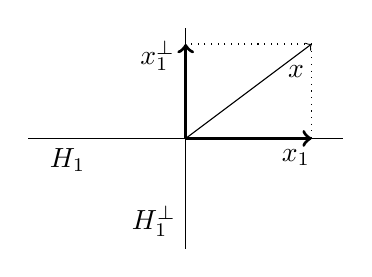
\begin{tikzpicture}[scale=0.2]
    \draw[solid] (-10, 0) --node[anchor=north, very near start]{$H_1$} (10, 0);
    \draw[solid] (0, -7) --node[anchor=east, very near start]{$H_1^\bot$} (0, 7);
    \draw[->] (0, 0) --node[anchor=north, very near end]{$x$} (8, 6);
    \draw[dotted](8, 6) -- (8, 0);
    \draw[dotted](8, 6) -- (0, 6);
    \draw[very thick, ->] (0, 0) -- node[anchor=north, very near end]{$x_1$} (8, 0);
    \draw[very thick, ->] (0, 0) -- node[anchor=east, very near end]{$x_1^\bot$} (0, 6);
\end{tikzpicture}


\subsection*{Ортогональные ряды.}

\noindent \textbullet~Пусть есть $\{ e_j \}$ - ОНС. Мы хотим понять, при каком условии $\forall x \; \norm{x}^2 = \sum \abs{(x, e_j)}^2$ - выполняется уравнение замкнутости.
Для этого рассмотрим ортогональный ряд $\sigma(x) = \sum_1^\infty (x, e_j) e_j$ и установим критерий сходимости. 

\bigskip 
\noindent\textbf{Утверждение \textnormal{(Критерий сходимости ортогонального ряда)}.} \textit{Пусть $H$ - гильбертовое пространство, $\sum_1^\infty x_j$ -
ортогональный ряд. Тогда он сходится $\Longleftrightarrow \sum_1^\infty \norm{x_j}^2 < +\infty$.} 

\begin{proof}

\smallskip
\noindent1)~Пусть ряд сходится $\Rightarrow \exists S = \lim_{n \to \infty} S_n$, $S_n = \sum_1^n x_j$. Из того, что $S_n \to S \Rightarrow \norm{S_n} \to \norm{S}$.
Сосчитаем квадрат нормы частичных сумм $\norm{S_n}^2 = \left(\sum_1^n x_j , \sum_1^n x_j\right) = \sum_{i, j = 1}^n (x_i, x_j)$, где если $i \neq j \Rightarrow = 0$.
Тогда $\norm{S_n}^2 = \sum_1^n \norm{x_j}^2 \to \norm{S}^2$. Поскольку $\sum_1^n \norm{x_j}^2$ - частичная сумма $\sum_1^\infty \norm{x_k}^2$, значит сходится. 

\medskip
\noindent \textbullet~Также в силу того, что есть соотношение $\sum_1^n \norm{x_j}^2 \to \norm{S}^2$ приходим, что $\norm{\sum_1^\infty x_j}^2 = \sum_1^\infty \norm{x_j}^2$
, что можно назвать теоремой Пифагора, для пространства гильберта.

\noindent2)~Пусть $\sum_1^\infty \norm{x_k}^2 < +\infty$. Тогда $\norm{S_{n+p} - S_n}^2 = \norm{\sum_{k = n + 1}^{n + p} x_k}^2$. Точно также как считалось выше за счет 
ортогональности $\norm{\sum_{k = n + 1}^{n + p} x_k}^2 = \sum_{k = n + 1}^{n+p} \norm{x_k}^2 \to 0$, $n, p \to \infty$ поскольку числовой ряд из квадратов норм сходится.
В результе получаем, что $\norm{S_{n +p} - S_n} \to 0$, а по полноте $H$ $\exists S = \lim S_n$. Доказано.
\end{proof}